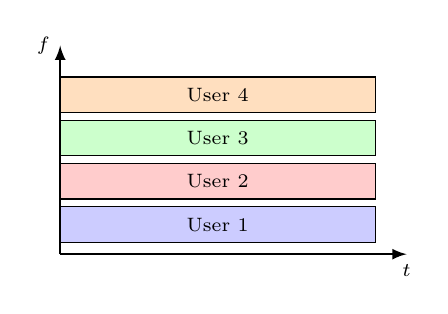
\begin{tikzpicture}[>=latex]
    \foreach \u/\col in {0/blue!20, 1/red!20, 2/green!20, 3/orange!25} {
        \draw[fill=\col] (0,{0.15+0.55*\u}) rectangle (4,{0.6+0.55*\u});
        \pgfmathtruncatemacro{\usernum}{\u+1}
        \node[font=\scriptsize] at (2,{0.375+0.55*\u}) {User \usernum};
    }
    \draw[->, thick] (0,0) -- (4.4,0) node[below, font=\scriptsize] {$t$};
    \draw[->, thick] (0,0) -- (0,2.65) node[left, font=\scriptsize] {$f$};
\end{tikzpicture}
